\documentclass[11pt]{article}
\usepackage[margin=1in]{geometry}
\usepackage{graphicx}
\usepackage{booktabs}
\usepackage{float}
\usepackage{hyperref}
\usepackage{amsmath}
\usepackage{array}

\title{SSD-Only Object Detection on a Traffic-Focused COCO Subset}
\author{Syed Aveed Ali}
\date{March 2, 2026}

\begin{document}
\maketitle

\begin{abstract}
This project implements an object detection pipeline based only on SSD (Single Shot MultiBox Detector), as required by the course constraint. The model is trained from scratch with \texttt{ssdlite320\_mobilenet\_v3\_large} on a six-class COCO-derived traffic dataset (\texttt{person}, \texttt{bicycle}, \texttt{car}, \texttt{motorcycle}, \texttt{bus}, \texttt{truck}). The training split contains 70,082 images and 332,526 annotated objects. With 5 training epochs on an NVIDIA RTX 4070 8GB GPU, the final validation score reached mAP@0.5:0.95 of 0.0925 and mAP@0.5 of 0.1876. Final held-out test results are mAP@0.5:0.95 = 0.0820, mAP@0.5 = 0.1715, precision = 0.5773, and recall = 0.2595. Measured inference speed is 33.64 FPS at 320\(\times\)320 input resolution. The report provides the full data pipeline, SSD formulation, implementation details, quantitative evaluation, and future improvements.
\end{abstract}

\section{Motivation}
Real-time object detection is critical in traffic-related computer vision tasks such as scene understanding, risk estimation, and autonomous perception. The challenge is to keep latency low while preserving detection quality across multiple object scales and classes.

The project goal is to build a detector with the following practical constraints:
\begin{itemize}
    \item use SSD only (no YOLO, no two-stage detector in the final model),
    \item train and evaluate on a realistic subset of COCO,
    \item produce reproducible training/evaluation artifacts and experiment logs.
\end{itemize}

SSD is appropriate for this setup because it performs localization and classification in one forward pass, making it computationally efficient. The expected trade-off is lower accuracy than heavier architectures, especially when classes are imbalanced or when training is short.

\section{Data}
\subsection{Dataset Source and Scope}
The dataset is built from COCO 2017 and converted to YOLO-format labels, then read by a custom PyTorch detection dataset class. The six classes are traffic-focused:
\texttt{person}, \texttt{bicycle}, \texttt{car}, \texttt{motorcycle}, \texttt{bus}, and \texttt{truck}.

\begin{table}[H]
\centering
\caption{Dataset split statistics}
\begin{tabular}{lrr}
\toprule
Split & Images & Objects \\
\midrule
Train & 70,082 & 332,526 \\
Validation & 1,484 & 7,037 \\
Test & 1,484 & 7,036 \\
\midrule
Total & 73,050 & 346,599 \\
\bottomrule
\end{tabular}
\end{table}

\subsection{Data Properties}
The dataset is strongly imbalanced. \texttt{person} dominates all splits, while \texttt{bus} and \texttt{bicycle} are much rarer. This class imbalance influences both training dynamics and metric behavior, typically improving precision on frequent classes before recall grows on minority classes.

\begin{figure}[H]
\centering
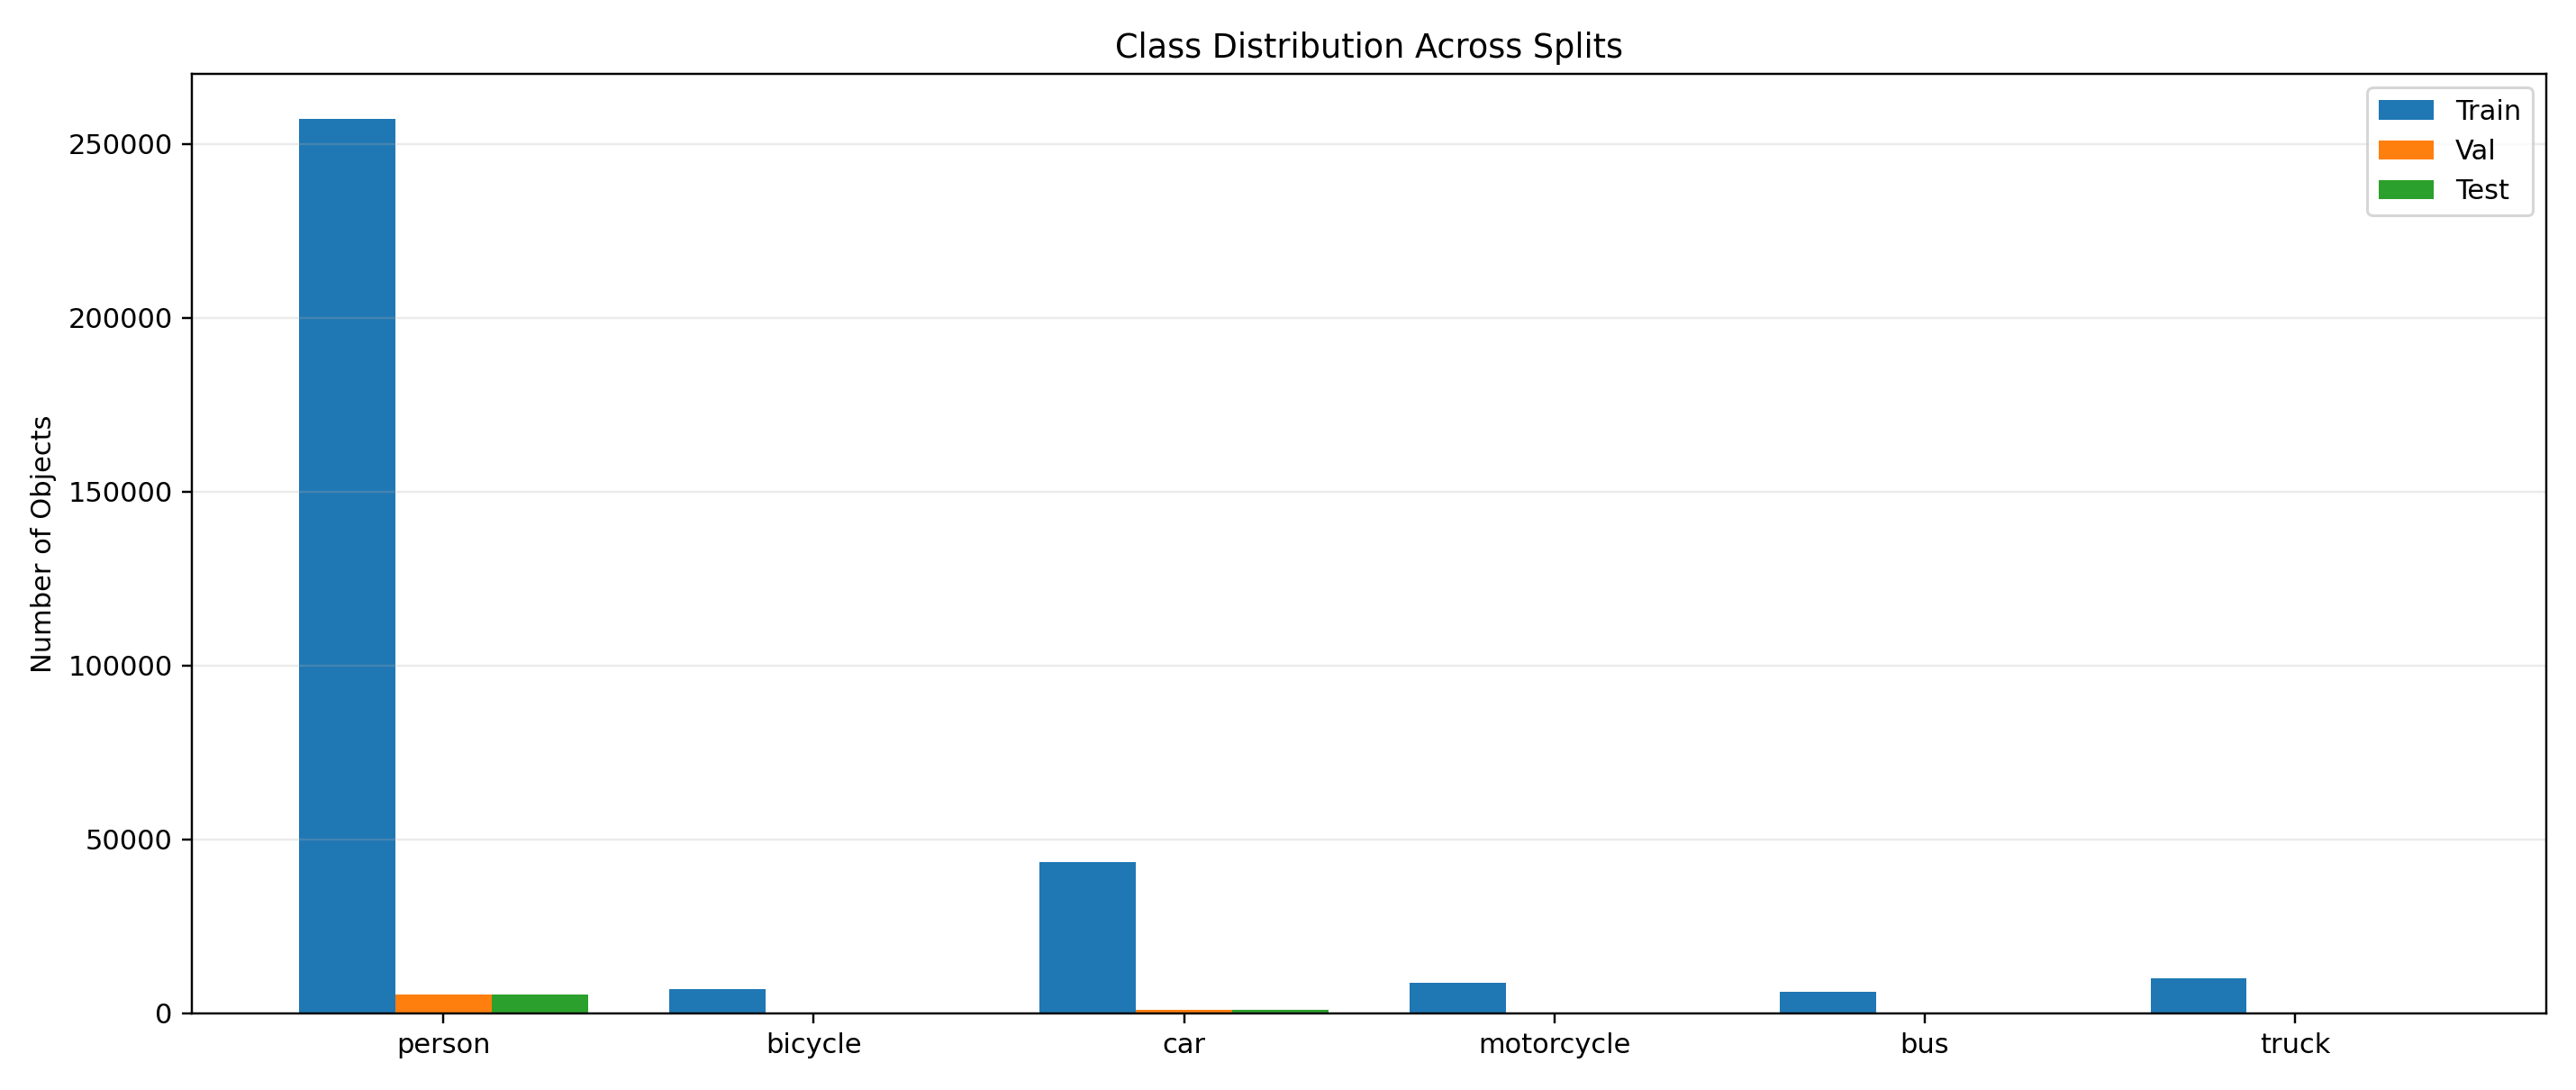
\includegraphics[width=0.97\textwidth]{figures/class_distribution.png}
\caption{Object count distribution across train/validation/test splits.}
\label{fig:class_dist}
\end{figure}

\subsection{Preprocessing and Augmentation}
The implemented preprocessing pipeline is lightweight and stable for SSD training:
\begin{itemize}
    \item resize images and boxes to 320\(\times\)320,
    \item random horizontal flip on training samples,
    \item conversion to normalized tensors,
    \item conversion from YOLO normalized \((x_c,y_c,w,h)\) to absolute \((x_1,y_1,x_2,y_2)\),
    \item class index shift by +1 for SSD background class 0.
\end{itemize}
No missing annotations were encountered during the final split used in this experiment.

\section{Theoretical Part and Literature Overview}
\subsection{Why SSD}
SSD \cite{liu2016ssd} is a one-stage detector that predicts class confidences and box offsets over default anchor boxes at multiple feature-map scales. Compared with two-stage detectors, SSD usually offers lower latency and simpler deployment. The hypothesis of this project is:

\begin{quote}
An SSD-Lite model with a mobile backbone can provide useful real-time traffic detection quality under limited GPU memory and training time.
\end{quote}

\subsection{Related Models}
Common alternatives include Faster R-CNN and YOLO-family models. Faster R-CNN often improves localization quality but is slower. YOLO variants are strong one-stage baselines but are outside the model-family constraint for this project. Therefore, the final system stays SSD-only.

\subsection{Learning Pipeline and Hyperparameters}
The SSD training pipeline follows:
\begin{enumerate}
    \item load YOLO-format dataset and transforms,
    \item initialize \texttt{ssdlite320\_mobilenet\_v3\_large} with random weights (from scratch),
    \item optimize with SGD (momentum 0.9, weight decay 5e-4),
    \item StepLR schedule (\(\gamma=0.1\), step at half training),
    \item evaluate each epoch with mAP, precision, recall,
    \item save \texttt{best.pth} by validation mAP@0.5:0.95.
\end{enumerate}

Main hyperparameters and expected impact:
\begin{itemize}
    \item \textbf{Input size (320)}: improves speed, may reduce small-object detail.
    \item \textbf{Batch size (16)}: stable on 8GB VRAM; larger batch may smooth gradients.
    \item \textbf{Epochs (5)}: fast experiment turnaround; likely under-trains rare classes.
    \item \textbf{Score threshold (0.25 in metrics, 0.40 in qualitative plots)}: controls precision-recall trade-off.
\end{itemize}

\section{Implementation}
\subsection{Code Structure}
The implementation is modular:
\begin{itemize}
    \item \texttt{coco\_det\_dataset.py}: dataset reader and YOLO-to-SSD target conversion,
    \item \texttt{transforms\_det.py}: resize/flip/tensor transforms for detection,
    \item \texttt{train\_ssd.py}: training loop, checkpointing, W\&B logging,
    \item \texttt{scripts/metrics\_det.py}: mAP and precision/recall computation,
    \item \texttt{scripts/evaluate\_ssd.py}: test-set evaluation,
    \item \texttt{scripts/benchmark\_ssd\_fps.py}: latency/FPS benchmark.
\end{itemize}

\subsection{Experiment Configuration}
Final training run used:
\begin{itemize}
    \item model: \texttt{ssdlite320\_mobilenet\_v3\_large},
    \item training mode: \textbf{from scratch},
    \item device: NVIDIA RTX 4070 8GB,
    \item epochs: 5,
    \item batch size: 16,
    \item optimizer: SGD, learning rate 0.002, momentum 0.9, weight decay 5e-4.
\end{itemize}

W\&B run link (public):
\url{https://wandb.ai/ahmadraza3195342-university-of-klagenfurt/ssd-course-project/runs/2lu80fwc}

\section{Evaluation}
\subsection{Validation Dynamics}
\begin{table}[H]
\centering
\caption{Per-epoch validation performance during training}
\begin{tabular}{rrrrrr}
\toprule
Epoch & Train Loss & mAP@0.5:0.95 & mAP@0.5 & Precision & Recall \\
\midrule
1 & 5.6090 & 0.0332 & 0.0880 & 0.2850 & 0.2215 \\
2 & 4.6991 & 0.0624 & 0.1382 & 0.5160 & 0.2295 \\
3 & 4.2635 & 0.0850 & 0.1770 & 0.5905 & 0.2555 \\
4 & 4.1851 & 0.0880 & 0.1808 & 0.5720 & 0.2672 \\
5 & 4.1240 & 0.0925 & 0.1876 & 0.5885 & 0.2680 \\
\bottomrule
\end{tabular}
\end{table}

\begin{figure}[H]
\centering
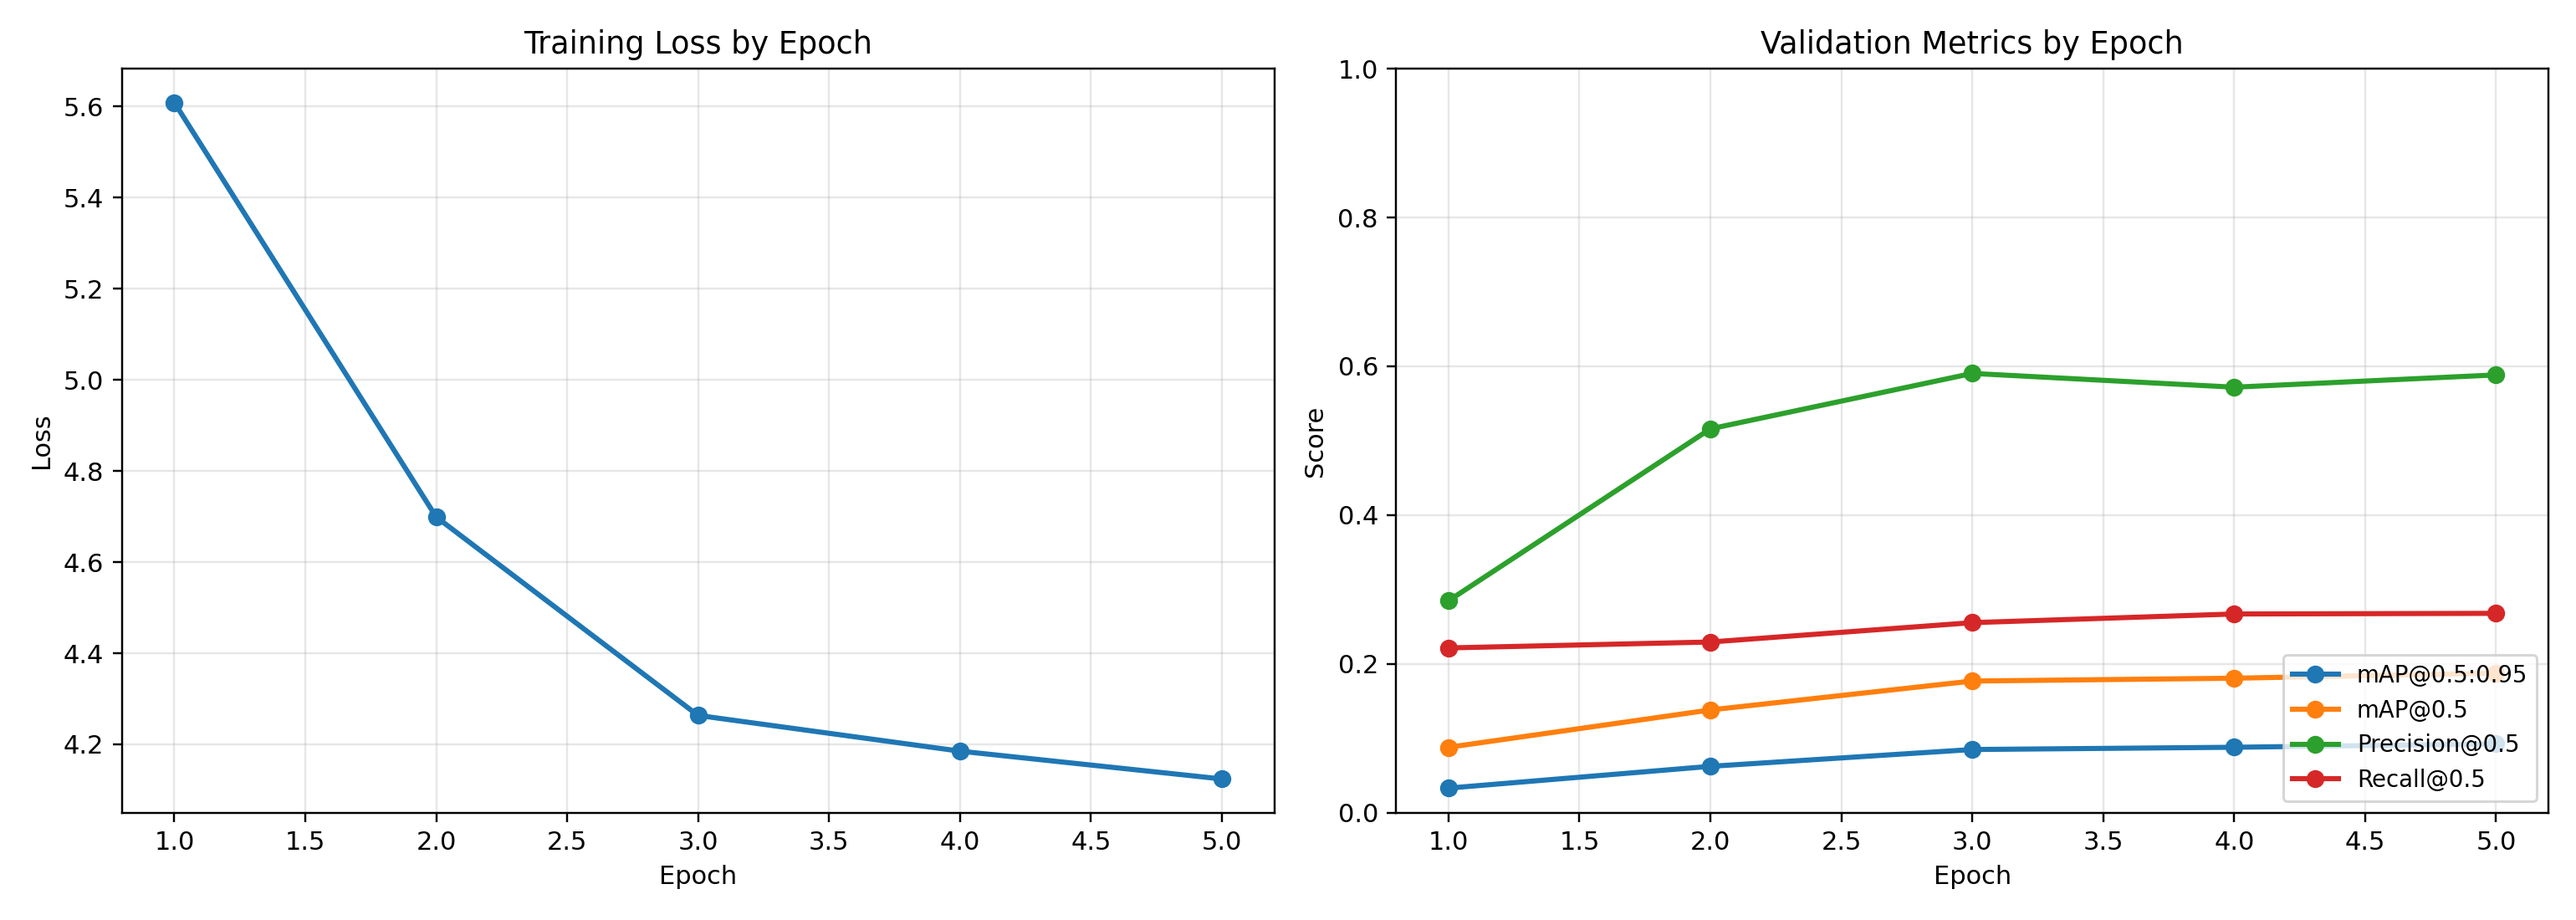
\includegraphics[width=0.97\textwidth]{figures/training_curves.png}
\caption{Training loss and validation metric curves over 5 epochs.}
\label{fig:curves}
\end{figure}

\subsection{Test-Set Results and Speed}
The best checkpoint (selected by validation mAP@0.5:0.95) was evaluated on the held-out test split.

\begin{table}[H]
\centering
\caption{Final SSD test metrics and inference speed}
\begin{tabular}{lrrrrr}
\toprule
Model & mAP@0.5:0.95 & mAP@0.5 & Precision & Recall & FPS \\
\midrule
SSD-Lite (best epoch) & 0.0820 & 0.1715 & 0.5773 & 0.2595 & 33.64 \\
\bottomrule
\end{tabular}
\end{table}

\subsection{Baseline Comparison}
An implemented baseline is the same model after epoch 1. Compared with epoch 1, the final epoch improves:
\begin{itemize}
    \item mAP@0.5:0.95 from 0.0332 to 0.0925 (+0.0593),
    \item mAP@0.5 from 0.0880 to 0.1876 (+0.0996),
    \item recall from 0.2215 to 0.2680 (+0.0465).
\end{itemize}
This confirms that even a short continuation from epoch 1 to epoch 5 yields clear gains.

\subsection{Qualitative Results}
\begin{figure}[H]
\centering
\includegraphics[width=0.97\textwidth]{figures/gt_samples.png}
\caption{Ground-truth annotations on sample test images.}
\label{fig:gt}
\end{figure}

\begin{figure}[H]
\centering
\includegraphics[width=0.97\textwidth]{figures/pred_samples.png}
\caption{SSD predictions on the same test images (score threshold 0.40).}
\label{fig:pred}
\end{figure}

Qualitatively, the detector is reliable on large and medium objects, especially \texttt{person} and \texttt{car}. Errors mostly appear on small, crowded scenes and minority classes (\texttt{bus}, \texttt{bicycle}), consistent with the class imbalance in Figure~\ref{fig:class_dist}.

\section{Conclusions}
This project delivered a complete SSD-only object detection pipeline with reproducible training, evaluation, and experiment tracking. The model achieved real-time throughput (33.64 FPS) with moderate detection quality after only 5 epochs from scratch.

Main takeaways:
\begin{itemize}
    \item SSD-Lite is practical under memory and latency constraints.
    \item Class imbalance strongly limits recall growth on rare classes.
    \item Additional training budget is likely the most direct next improvement.
\end{itemize}

Recommended future steps:
\begin{itemize}
    \item train longer (30--100 epochs) with stronger augmentation,
    \item evaluate class-weighted or focal-style loss variants,
    \item tune score/NMS thresholds and per-class confidence thresholds,
    \item perform a controlled comparison against SSD with pretrained backbone for the same dataset.
\end{itemize}

\begin{thebibliography}{9}
\bibitem{liu2016ssd}
W. Liu, D. Anguelov, D. Erhan, C. Szegedy, S. Reed, C.-Y. Fu, and A. C. Berg,
\emph{SSD: Single Shot MultiBox Detector}, ECCV, 2016.

\bibitem{lin2014coco}
T.-Y. Lin, M. Maire, S. Belongie, et al.,
\emph{Microsoft COCO: Common Objects in Context}, ECCV, 2014.

\bibitem{mobilenetv3}
A. Howard, M. Sandler, G. Chu, et al.,
\emph{Searching for MobileNetV3}, ICCV, 2019.
\end{thebibliography}

\end{document}
